\section{Results}

\subsection{Puck}
This part was chosen as a first simulation because of its simplicity.  The puck acts just as a part that can be simulated to find out whether the simulation setup and the refinement algorithm work.  There is no industrial motivation for simulating this part, just a need to verify that all scripts work and that the simulation will run without crashing.  

\subsubsection{Setup}
The puck was constructed with a diameter of 5mm and a height of 3mm.  The voxelized mesh was created to balance run time and fidelity to the original shape.  Thus, a mesh of 0.5mm was used for the part under test, and the "base" was given a coarser mesh of 2mm.  

\subsubsection{Results}
An image of the final stress result is shown below.
\begin{figure}[H]
    \centering
    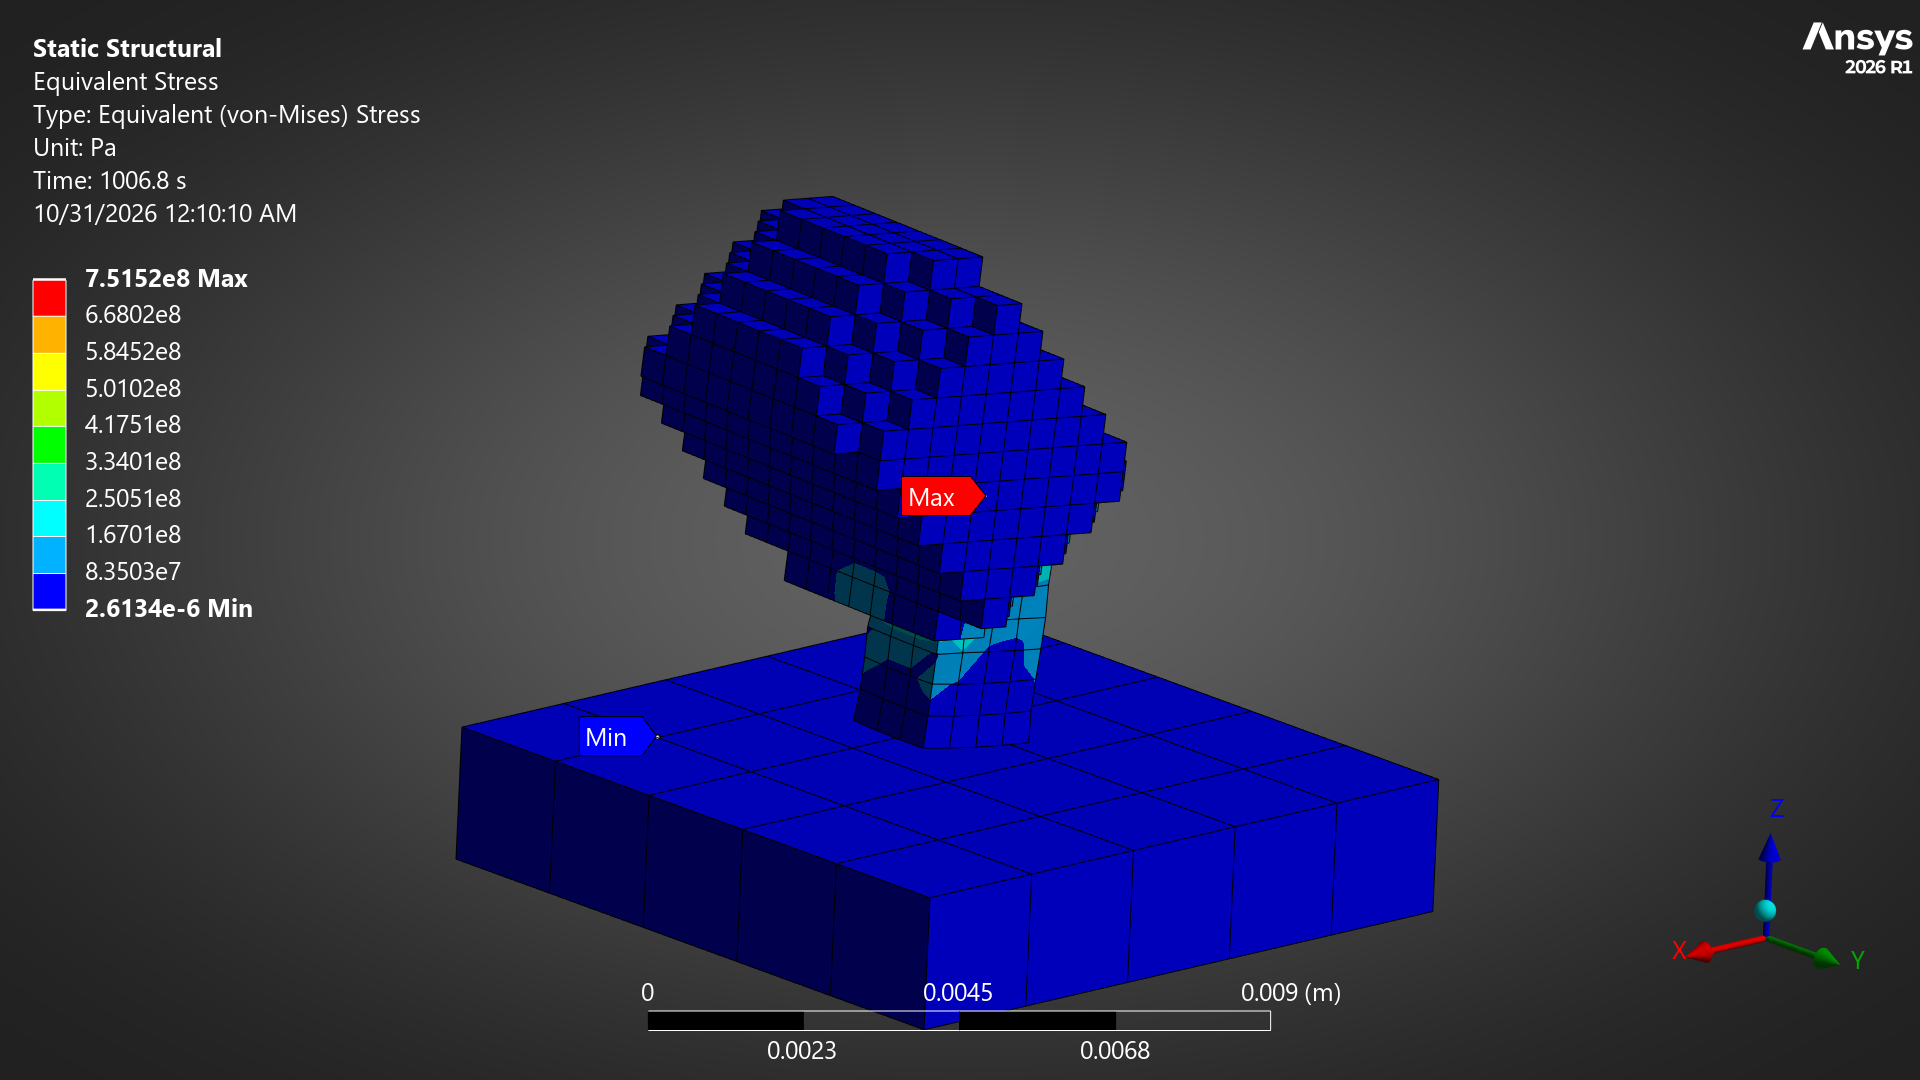
\includegraphics[width=1\linewidth]{Figures/Results/Puck/results/bo_037_equivalent_stress.png}
    \caption[The final stress result of the simulated puck.]{The final stress result of the simulated puck.}
    \label{fig:Puck Final Stress}
\end{figure}

This was the final rotation after a full run of stress optimization.
\begin{figure}[H]
    \centering
    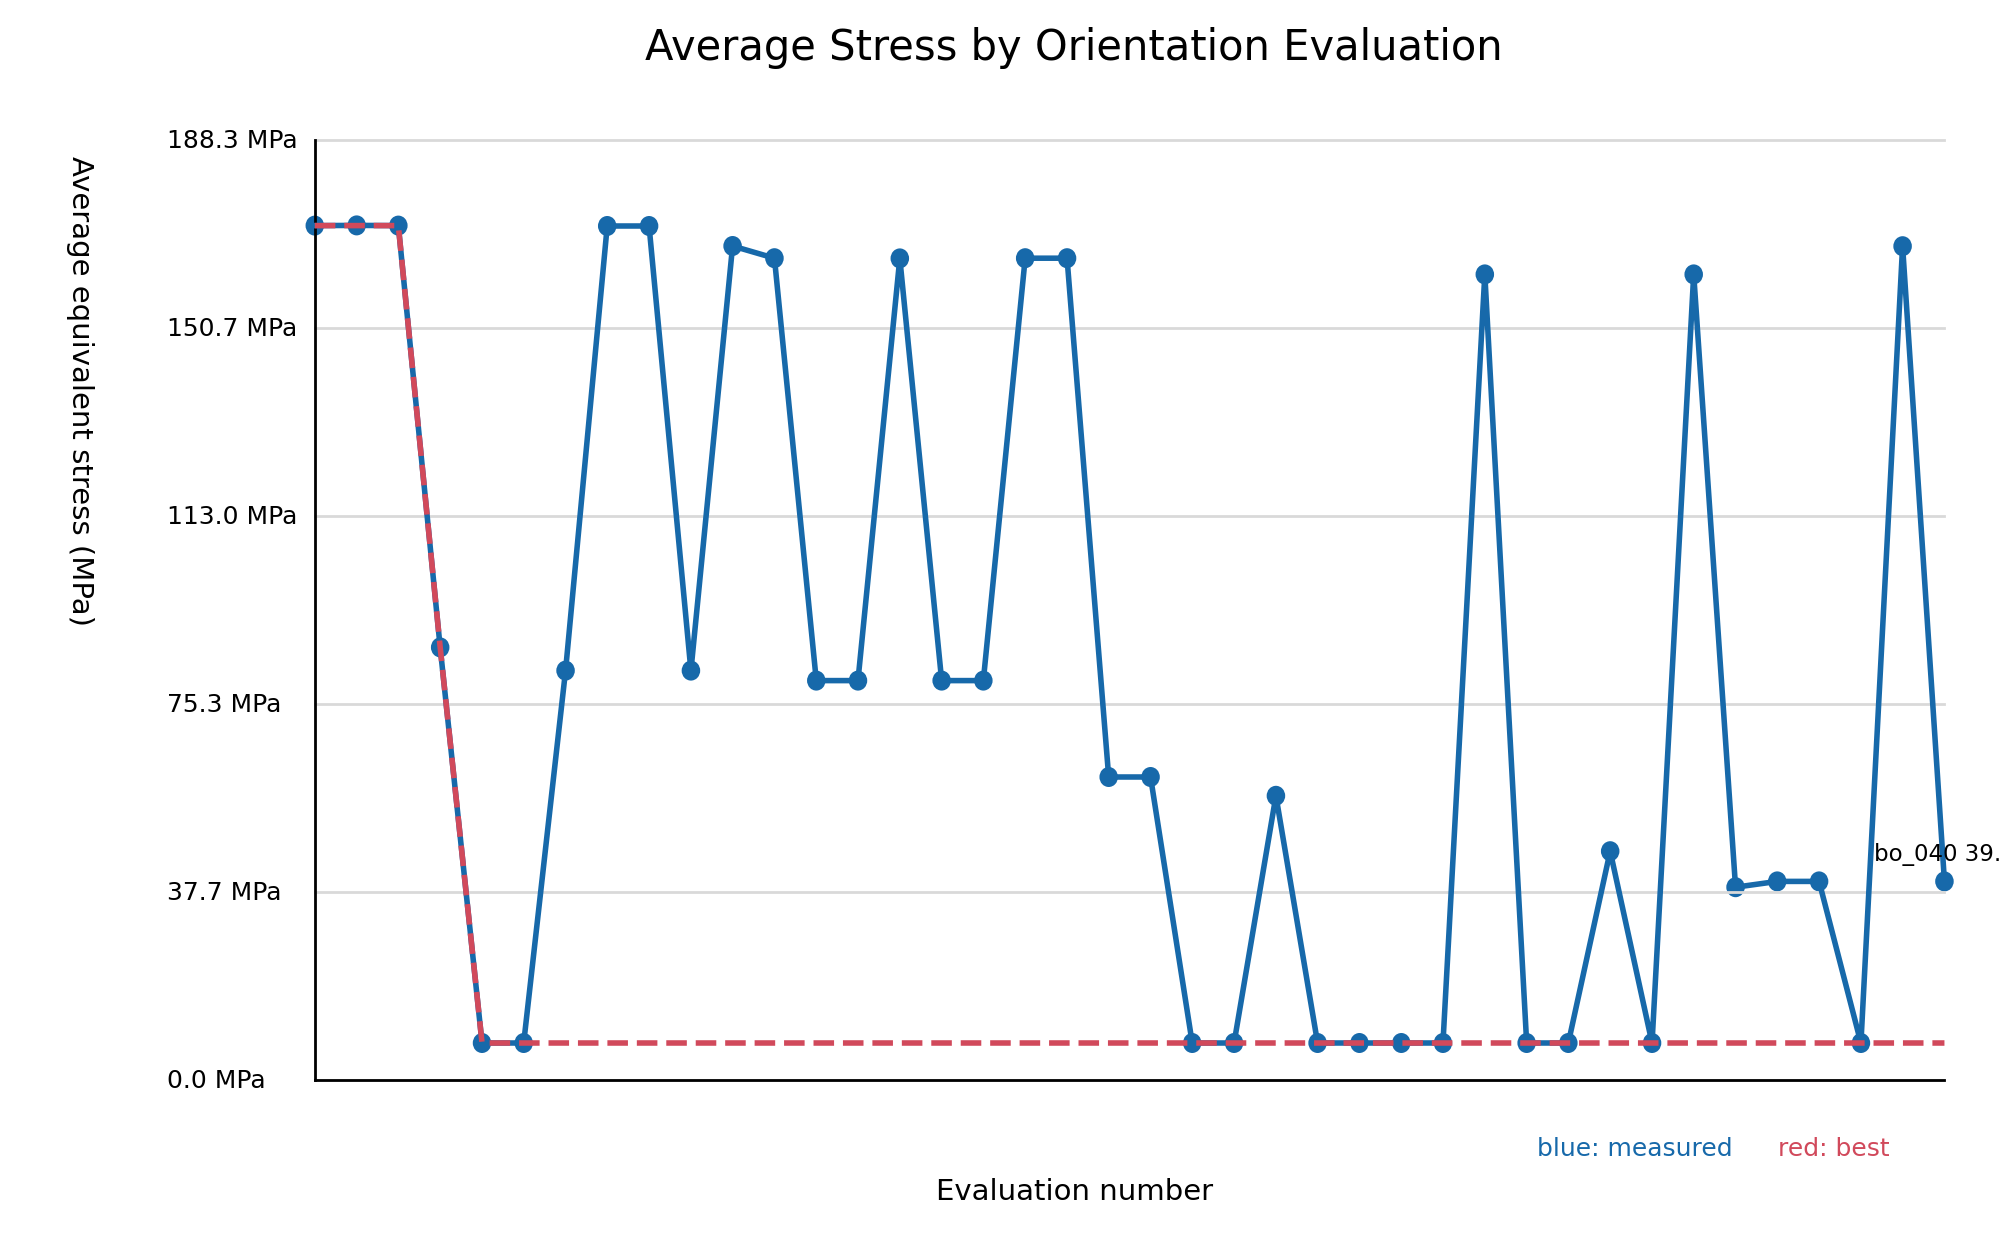
\includegraphics[width=1\columnwidth]{Figures/Results/Puck/results/stress_progress.png}
    \caption[The graph showing the progression of average stress over the run's iterations.]{The graph showing the progression of average stress over the run's iterations.}
    \label{fig:Puck Stress Graph}
\end{figure}

\begin{figure}[H]
	\centering
	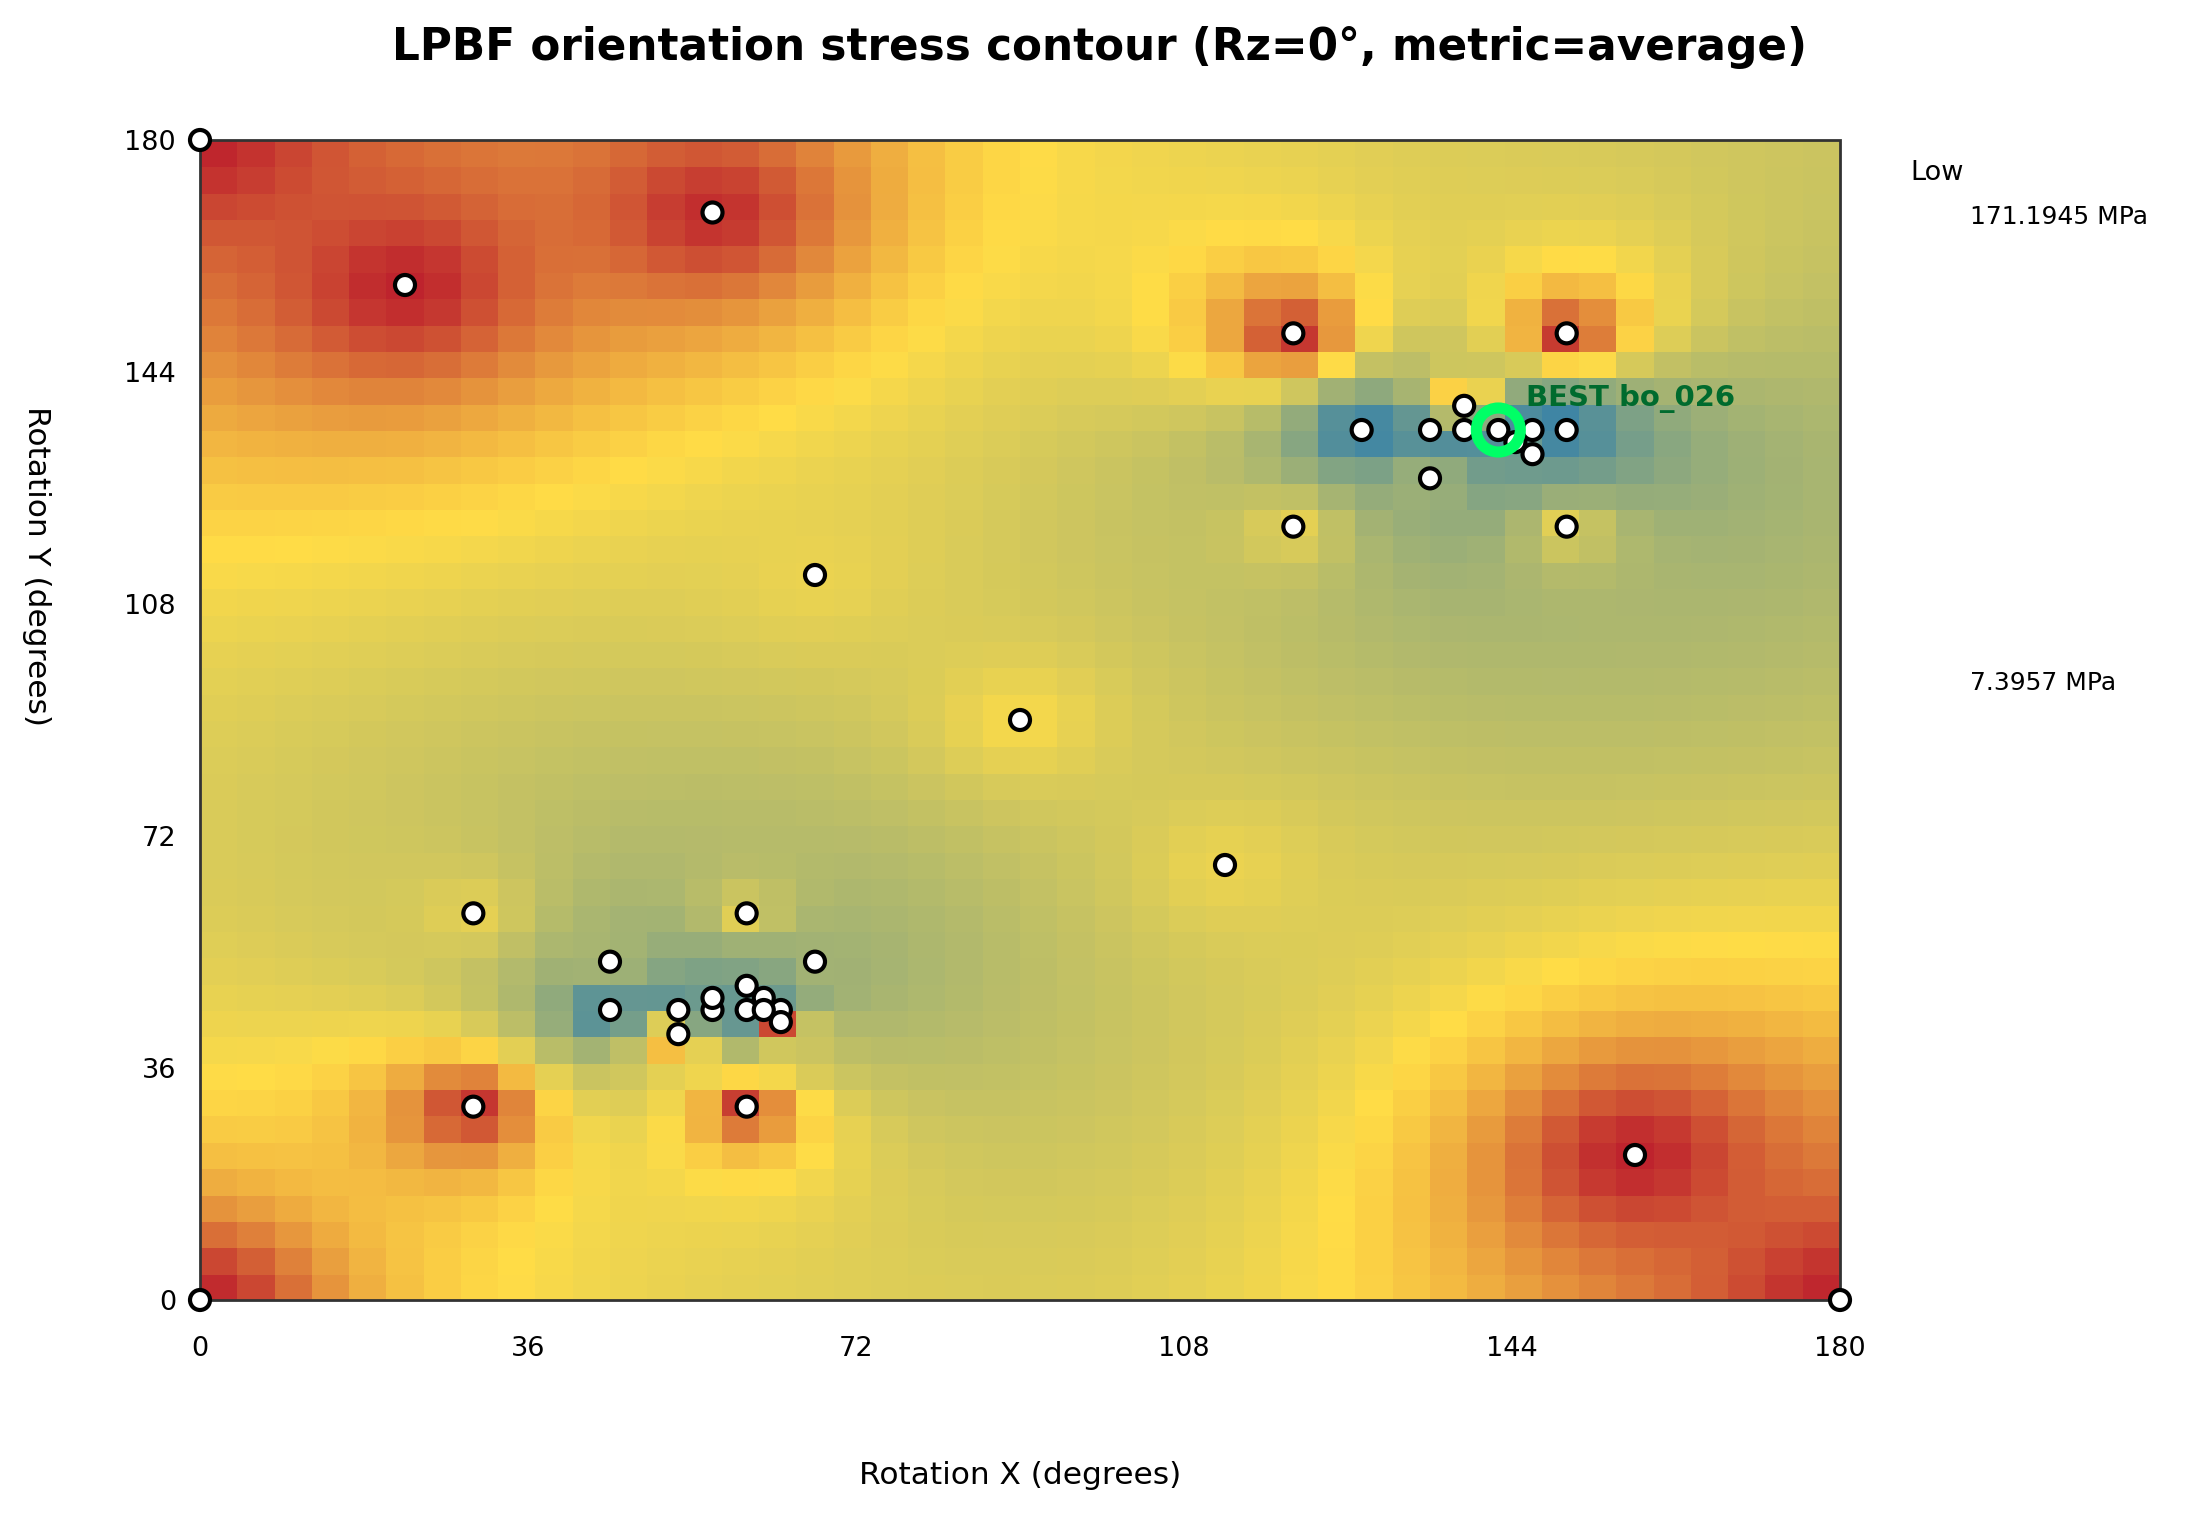
\includegraphics[width=1\columnwidth]{Figures/Results/Puck/results/orientation_contour_map.png}
	\caption[A contour map of the stress vs. rotation angle.  Note the data is quite sparse, so graph usefulness may be questionable.]{A contour map of the stress vs. rotation angle.  Note the data is quite sparse, so graph usefulness may be questionable.}
	\label{fig:Puck Stress Contour}
\end{figure}


For this run, when looking at \ref{fig:Puck Stress Graph}, it can be seen that the stress bottomed out relatively early in the run.  The algorithm took this location into account, and continued to run the original "seed" simulations, to get an awareness of the design space.  Once those runs were done, the search went back to the area around the minimum stress already found, resulting in \ref{fig:Puck Final Stress}.  Then it searched around the area.  The step is $15^\circ$ and the program explored around that area.  It found a few rotation points that were higher, and moved away from them.  Eventually, after a number of iterations (find that info) around the minimum stress point, there was no notable improvement.  Thus, the criteria was met to end the simulation (find this out too).  
\newline \indent Through this simulation, it was found that the optimal orientation is a rotation of $\theta_x =61^\circ$ and $theta_x=45^\circ$ to have the optimal stress.  This result could have been found quicker than this graph shows if the criteria were loosened, but that is not always the case.  There is also a sort of contour map in

\subsection{Compressor Wheel}

\begin{figure}[H]
	\centering
	\includegraphics[width=1\linewidth]{Figures/Results/Compressor wheel/Printed compressor wheel.png}
	\caption[A 3D printed compressor wheel]{A 3D printed compressor wheel \cite{AddUpImpellerWheel}.}
	\label{fig:Printed Compressor Wheel}
\end{figure}

\begin{figure}[H]
	\centering
	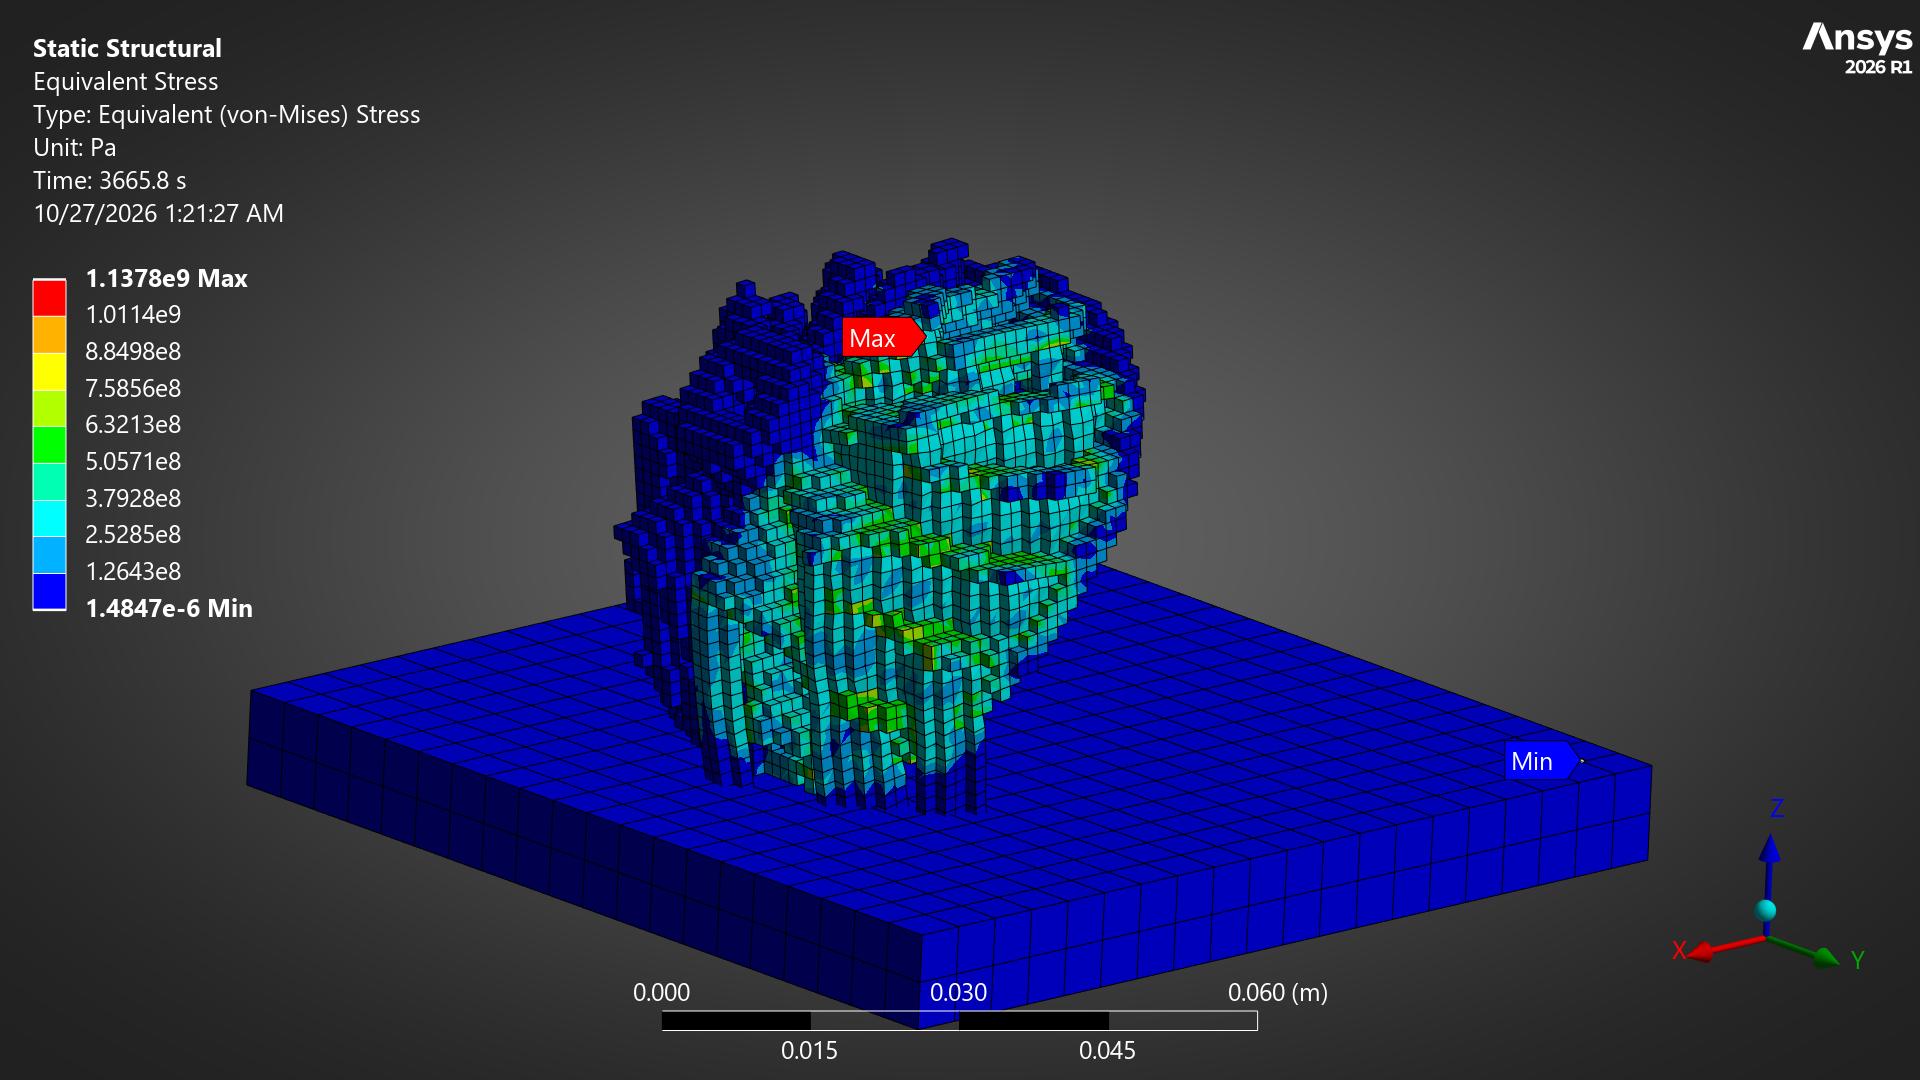
\includegraphics[width=1\linewidth]{Figures/Results/Compressor wheel/results/bo_020_equivalent_stress.png}
	\caption[The final stress result of the simulated compressor wheel]{The final stress result of the simulated compressor wheel.}
	\label{fig:Compressor Wheel Final Stress}
	\end{figure}

This was the final rotation after a full run of stress optimization.
\begin{figure}[H]
	\centering
	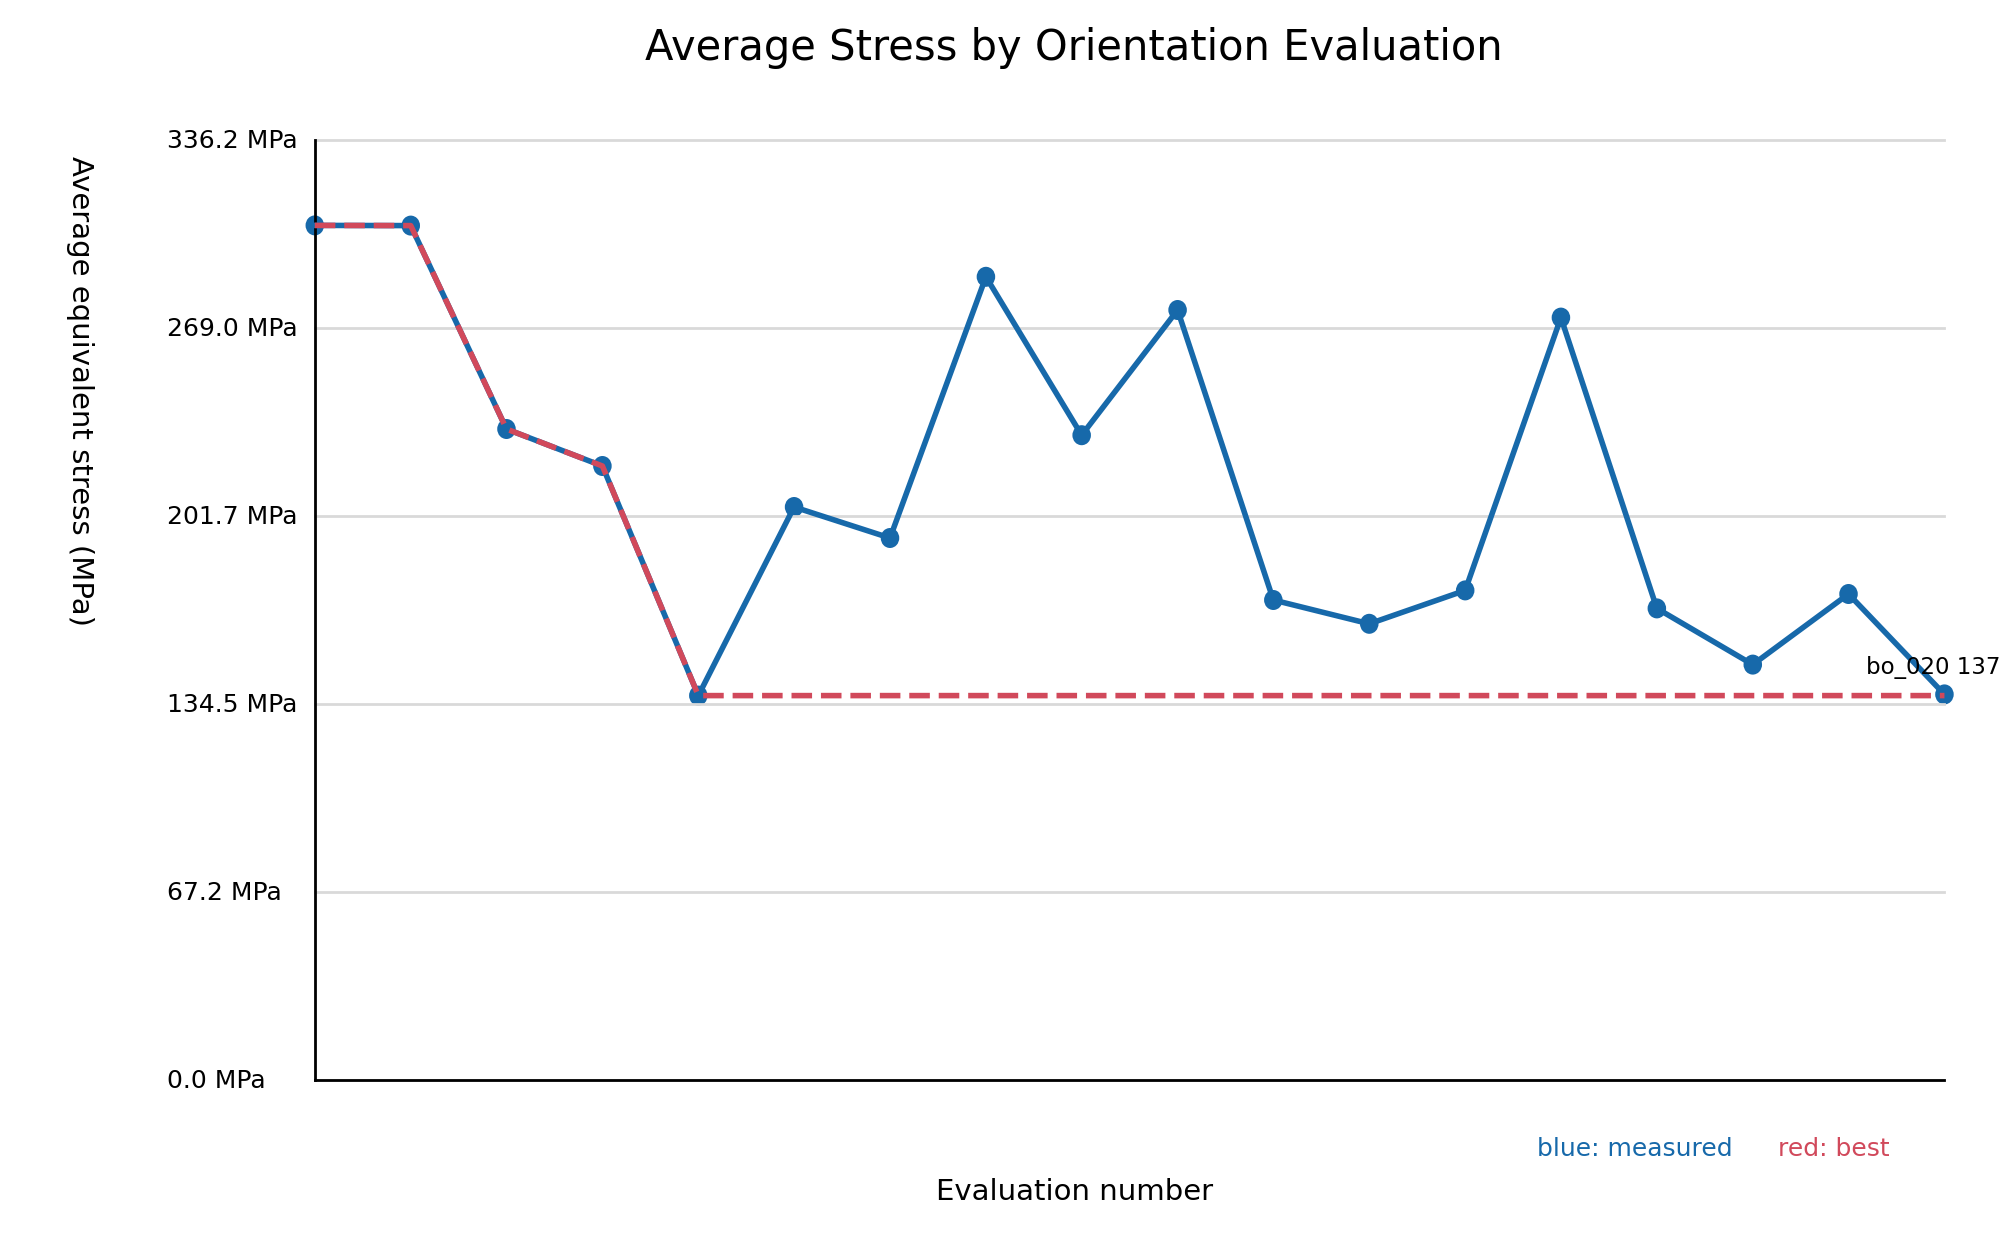
\includegraphics[width=1\columnwidth]{Figures/Results/Compressor wheel/results/stress_progress.png}
	\caption[The graph showing the progression of average stress over the run's iterations.]{The graph showing the progression of average stress over the run's iterations.}
	\label{fig:Compressor Wheel Stress Graph}
\end{figure}

\begin{figure}[H]
	\centering
	\includegraphics[width=1\columnwidth]{Figures/Results/Compressor Wheel/results/orientation_contour_map.png}
	\caption[A contour map of the stress vs. rotation angle.  Note the data is quite sparse, so graph usefulness may be questionable.]{A contour map of the stress vs. rotation angle.  Note the data is quite sparse, so graph usefulness may be questionable.}
	\label{fig:Compressor Stress Contour}
\end{figure}

\subsubsection{Motivation}
Compressor wheels are an ever present part of air movement.  They most frequently show up in turbochargers for automotive purposes, but also make appearances in small jet engines.  They are frequently cast or machined.  Both of these processes are not optimal for mass manufacturing.  Machining these parts requires a large piece of round billet to start, out of which the majority of material is machined away, taking up significant machine time and wasting material.  Casting this part requires investment casting, due to the amount of overhangs in the part.  Investment casting has a large capital overhead and a high amount of tooling investment. The complex geometry and demands of spinning at 100,000 rpm brings AM into the question for this part.  The geometry simulated in this section was found on Grabcad, and is a stand-in for production geometry to show the capabilities of this software.

\subsubsection{Setup}
To set up this run, the geometry steps explained in Methodology were used.  Once the geometry was prepared, the run was started with a mesh of 1.5mm on the compressor wheel, and 5mm on the base.

\subsection{Turbine Blade}

\begin{figure}[H]
	\centering
	\includegraphics[width=1\linewidth]{Figures/Results/Turbine Blade/Turbine Blades.png}
	\caption[A 3D-printed turbine blade]{A 3D printed turbine blade \cite{Caiazzo2017LPBFTurbineBlades}}
	\label{fig:Printed Turbine Blade}
\end{figure}

\subsubsection{Motivation}
Turbine blades are one of the most difficult parts to manufacture on the market today.  They are found in the hot section of jet engines and gas turbines, and undergo tremendous loads through their lifetime.  In addition to constantly spinning around 5000rpm for hundreds or thousands of hours, they are subject to temperatures in excess of $1500^\circ C$ while spinning.  To remedy this problem, manufacturers have spent decades refining the casting process to grow blades that can retain their properties over their service life.  In addition to tight material properties and crystal growth control, there are tiny holes going through the blades.  These holes are no larger than 1mm in diameter, and go through 6 inches of blade.  This kind of intricate detail makes these blades difficult to cast and machine, and lends iself to LPBF, in which tight tolerances can be met.

\begin{figure}[H]
\centering
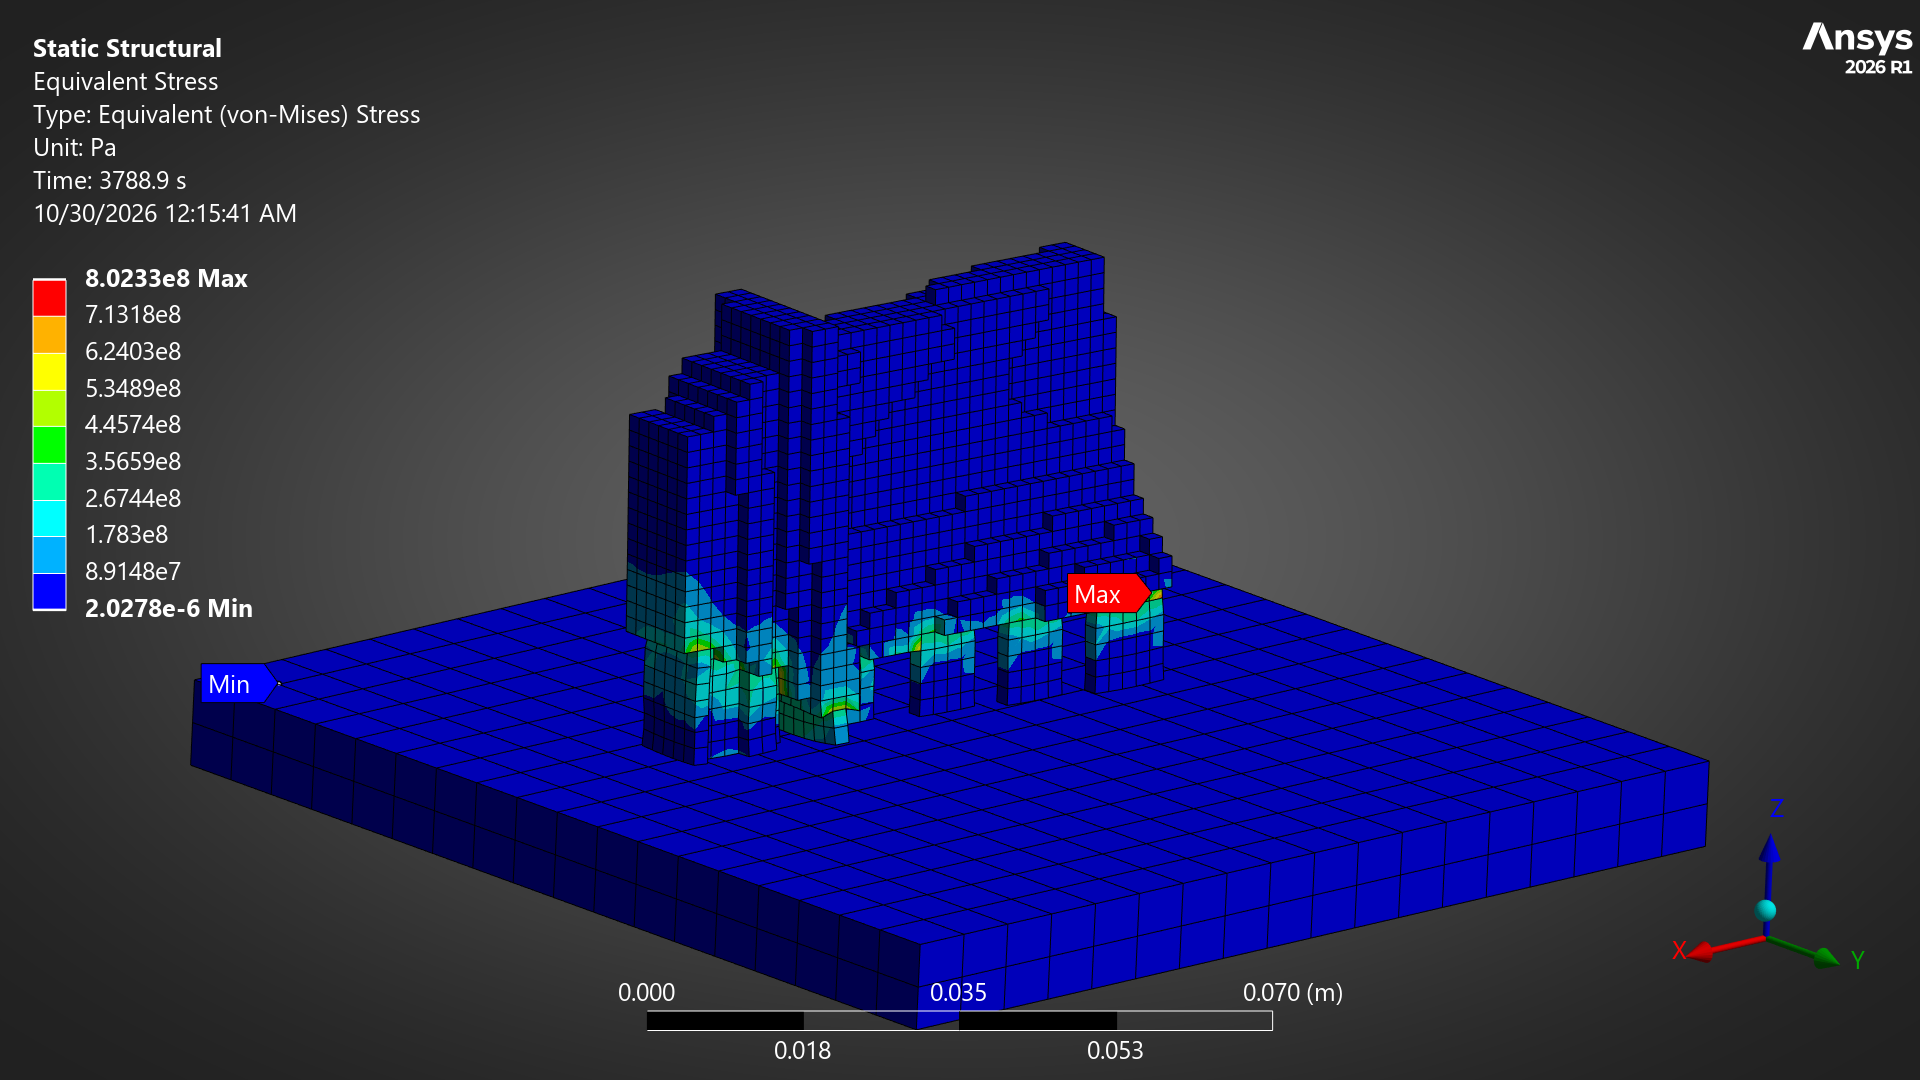
\includegraphics[width=1\linewidth]{Figures/Results/Turbine Blade/results/bo_060_equivalent_stress.png}
\caption[The final stress result of the simulated turbine blade]{The final stress result of the simulated turbine blade.}
\label{fig:Turbine Blade Final Stress}
\end{figure}

This was the final rotation after a full run of stress optimization.
\begin{figure}[H]
\centering
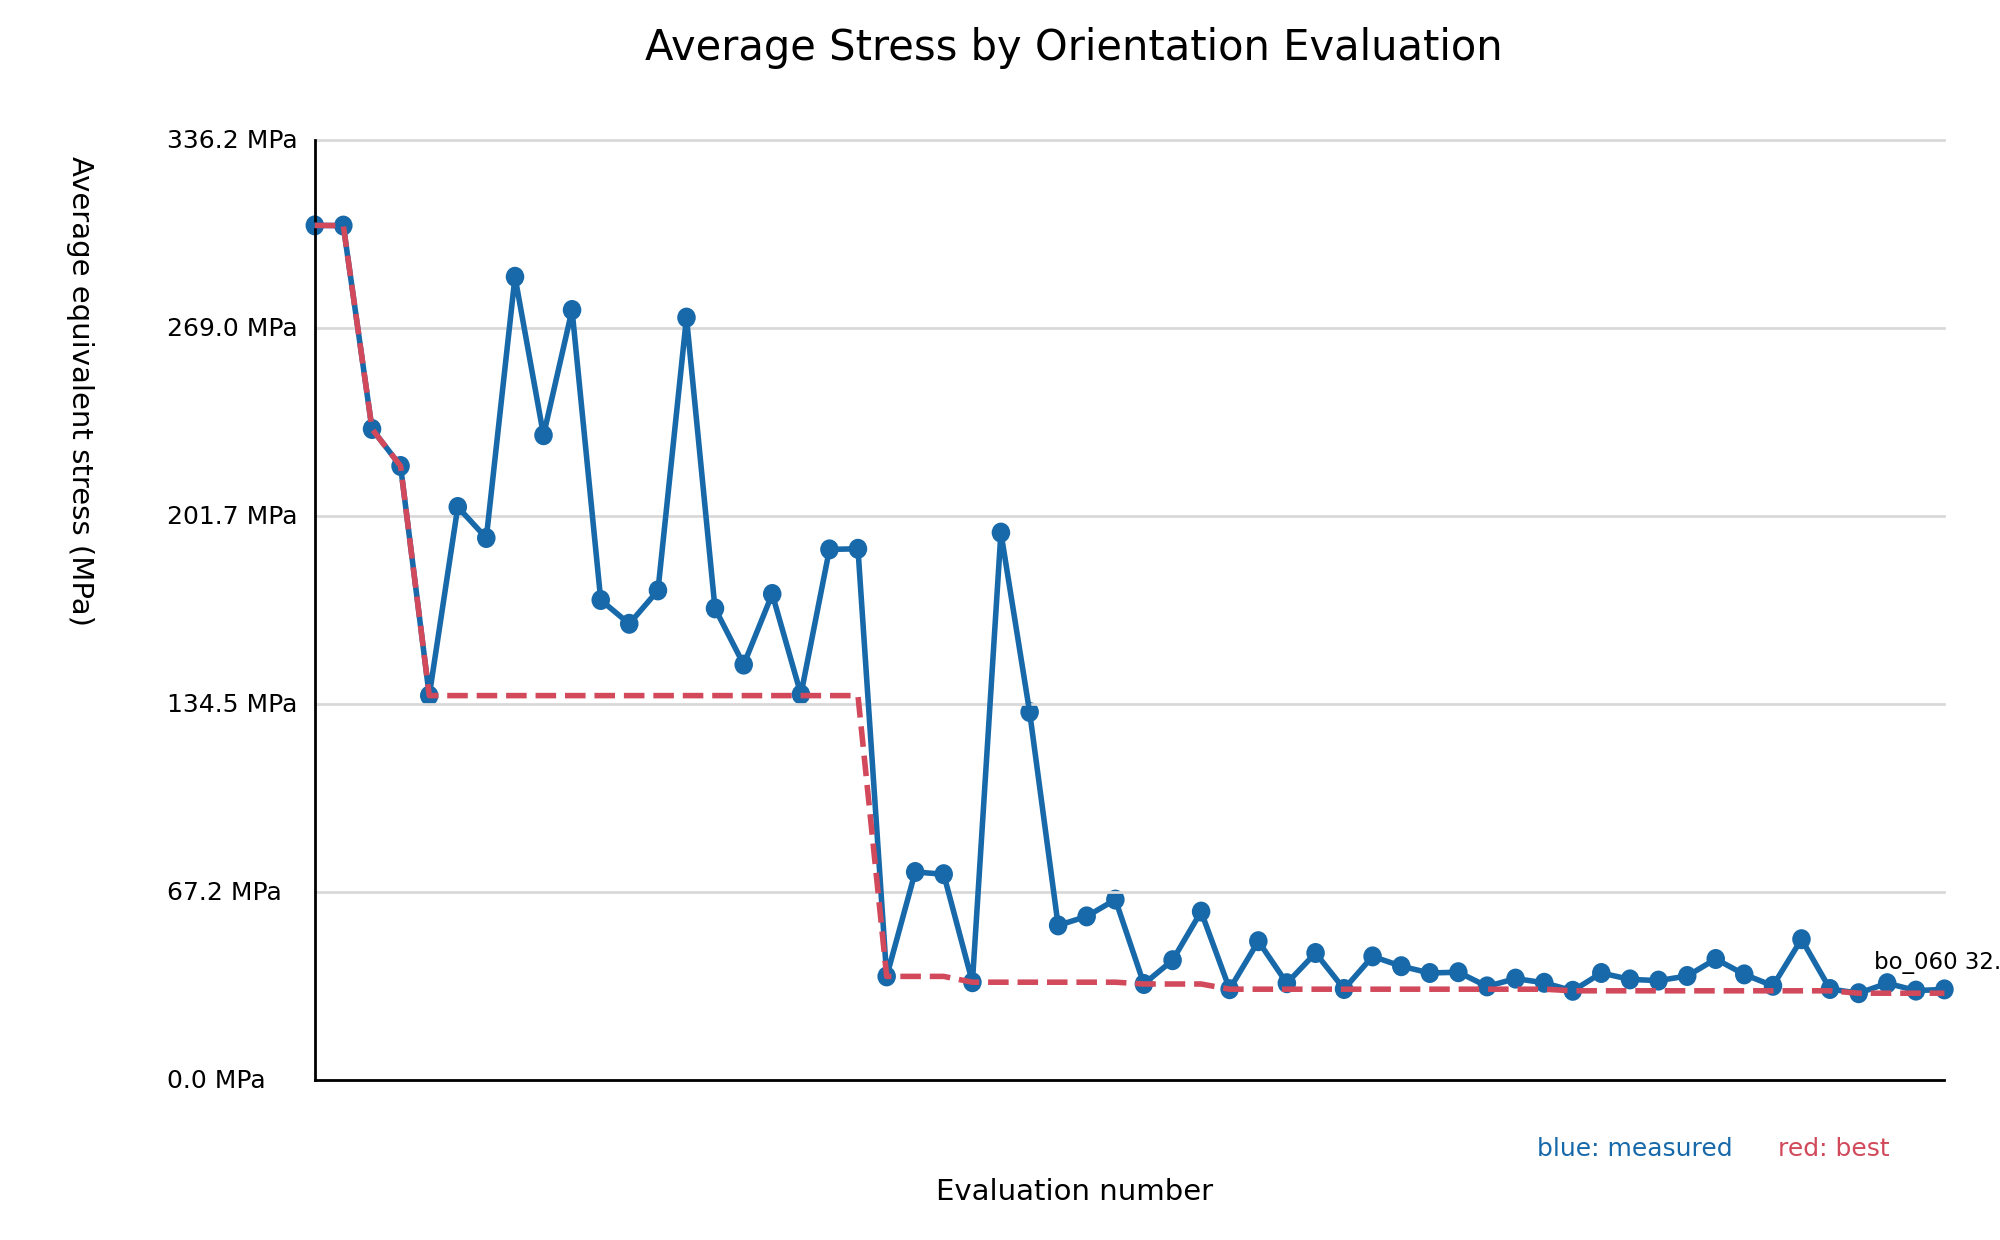
\includegraphics[width=1\columnwidth]{Figures/Results/Turbine Blade/results/stress_progress.png}
\caption[The graph showing the progression of average stress over the run's iterations.]{The graph showing the progression of average stress over the run's iterations.}
\label{fig:Turbine Blade Stress Graph}
\end{figure}

\begin{figure}[H]
	\centering
	\includegraphics[width=1\columnwidth]{Figures/Results/Turbine Blade/results/orientation_contour_map.png}
	\caption[A contour map of the stress vs. rotation angle.  Note the data is quite sparse, so graph usefulness may be questionable.]{A contour map of the stress vs. rotation angle.  Note the data is quite sparse, so graph usefulness may be questionable.}
	\label{fig:Turbine Blade Stress Contour}
\end{figure}

\subsubsection{Setup}

The geometry was preprocessed according to Section 2, and a mesh of 2mm was chosen, along with 10mm on the base.

\subsection{Exhaust Manifold}

\begin{figure}[H]
	\centering
	\includegraphics[width=1\linewidth]{Figures/Results/Exhaust Manifold/3d printed exhaust.png}
	\caption[A 3D printed exhaust manifold]{A 3D printed exhaust manifold \cite{Sher2020PapadakisTurboManifold}.}
	\label{fig:3D Printed Exhaust}
\end{figure}

\subsubsection{Motivation}
Exhaust manifolds are prime examples of a part with difficult geometry for manufacturing along with a high temperature requirement, being located just outside of the combustion chamber of a piston engine.  The common method of mass-manufacturing is casting, however, the sand molds need to be multi-piece to create the hollow sections for exhaust gases to flow through.  In lieu of mass production, exhaust manifolds are frequently made by cutting and bending pipe segments, then welding them together.  This is a process that requires great fabrication skill, and is often an expensive process of any custom engine build.  Recently, with this in mind, custom engine fabricators have begun to apply AM to exhaust manifolds, with multiple printable materials being able to handle the high temperatures this part is subject to.  


\begin{figure}[H]
	\centering
	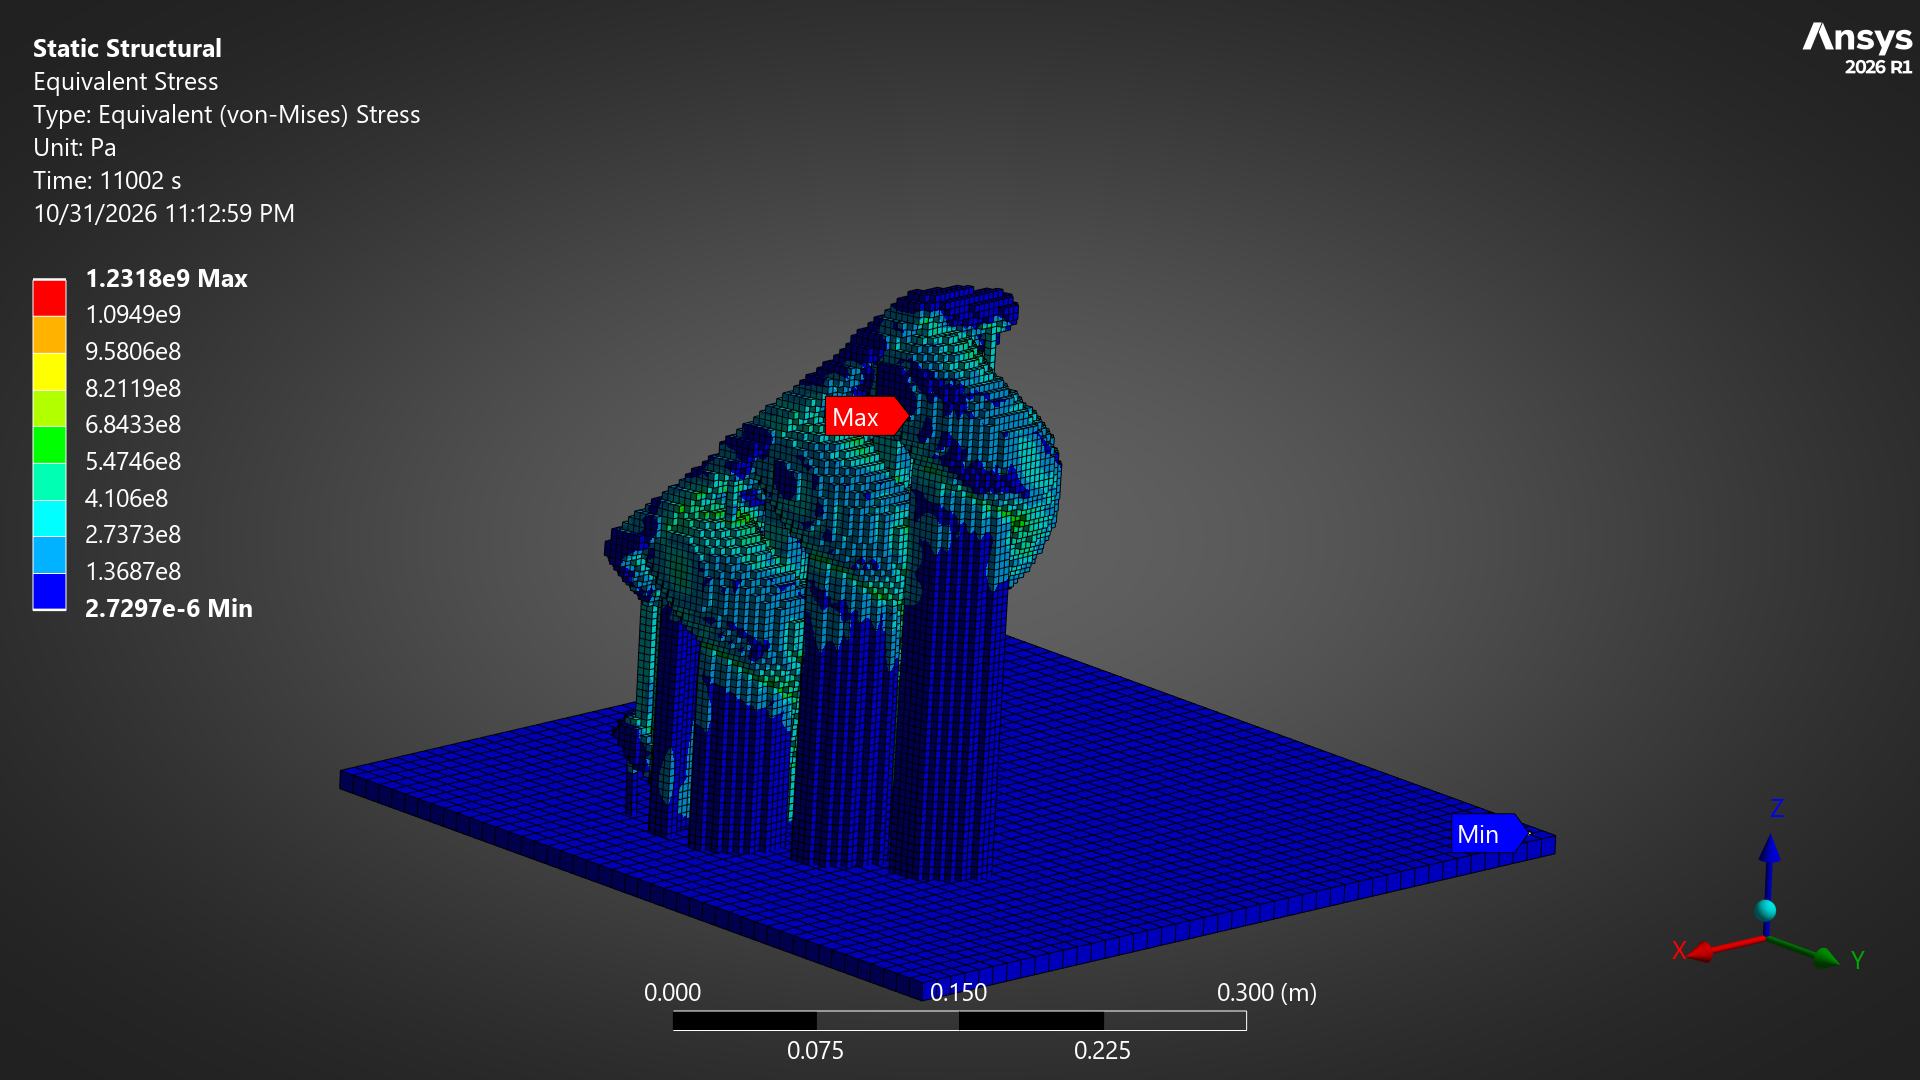
\includegraphics[width=1\linewidth]{Figures/Results/Exhaust Manifold/results/bo_024_equivalent_stress.png}
	\caption[The final stress result of the simulated exhaust manifold]{The final stress result of the simulated exhaust manifold.}
	\label{fig:Exhaust Manifold Final Stress}
\end{figure}

This was the final rotation after a full run of stress optimization.
\begin{figure}[H]
	\centering
	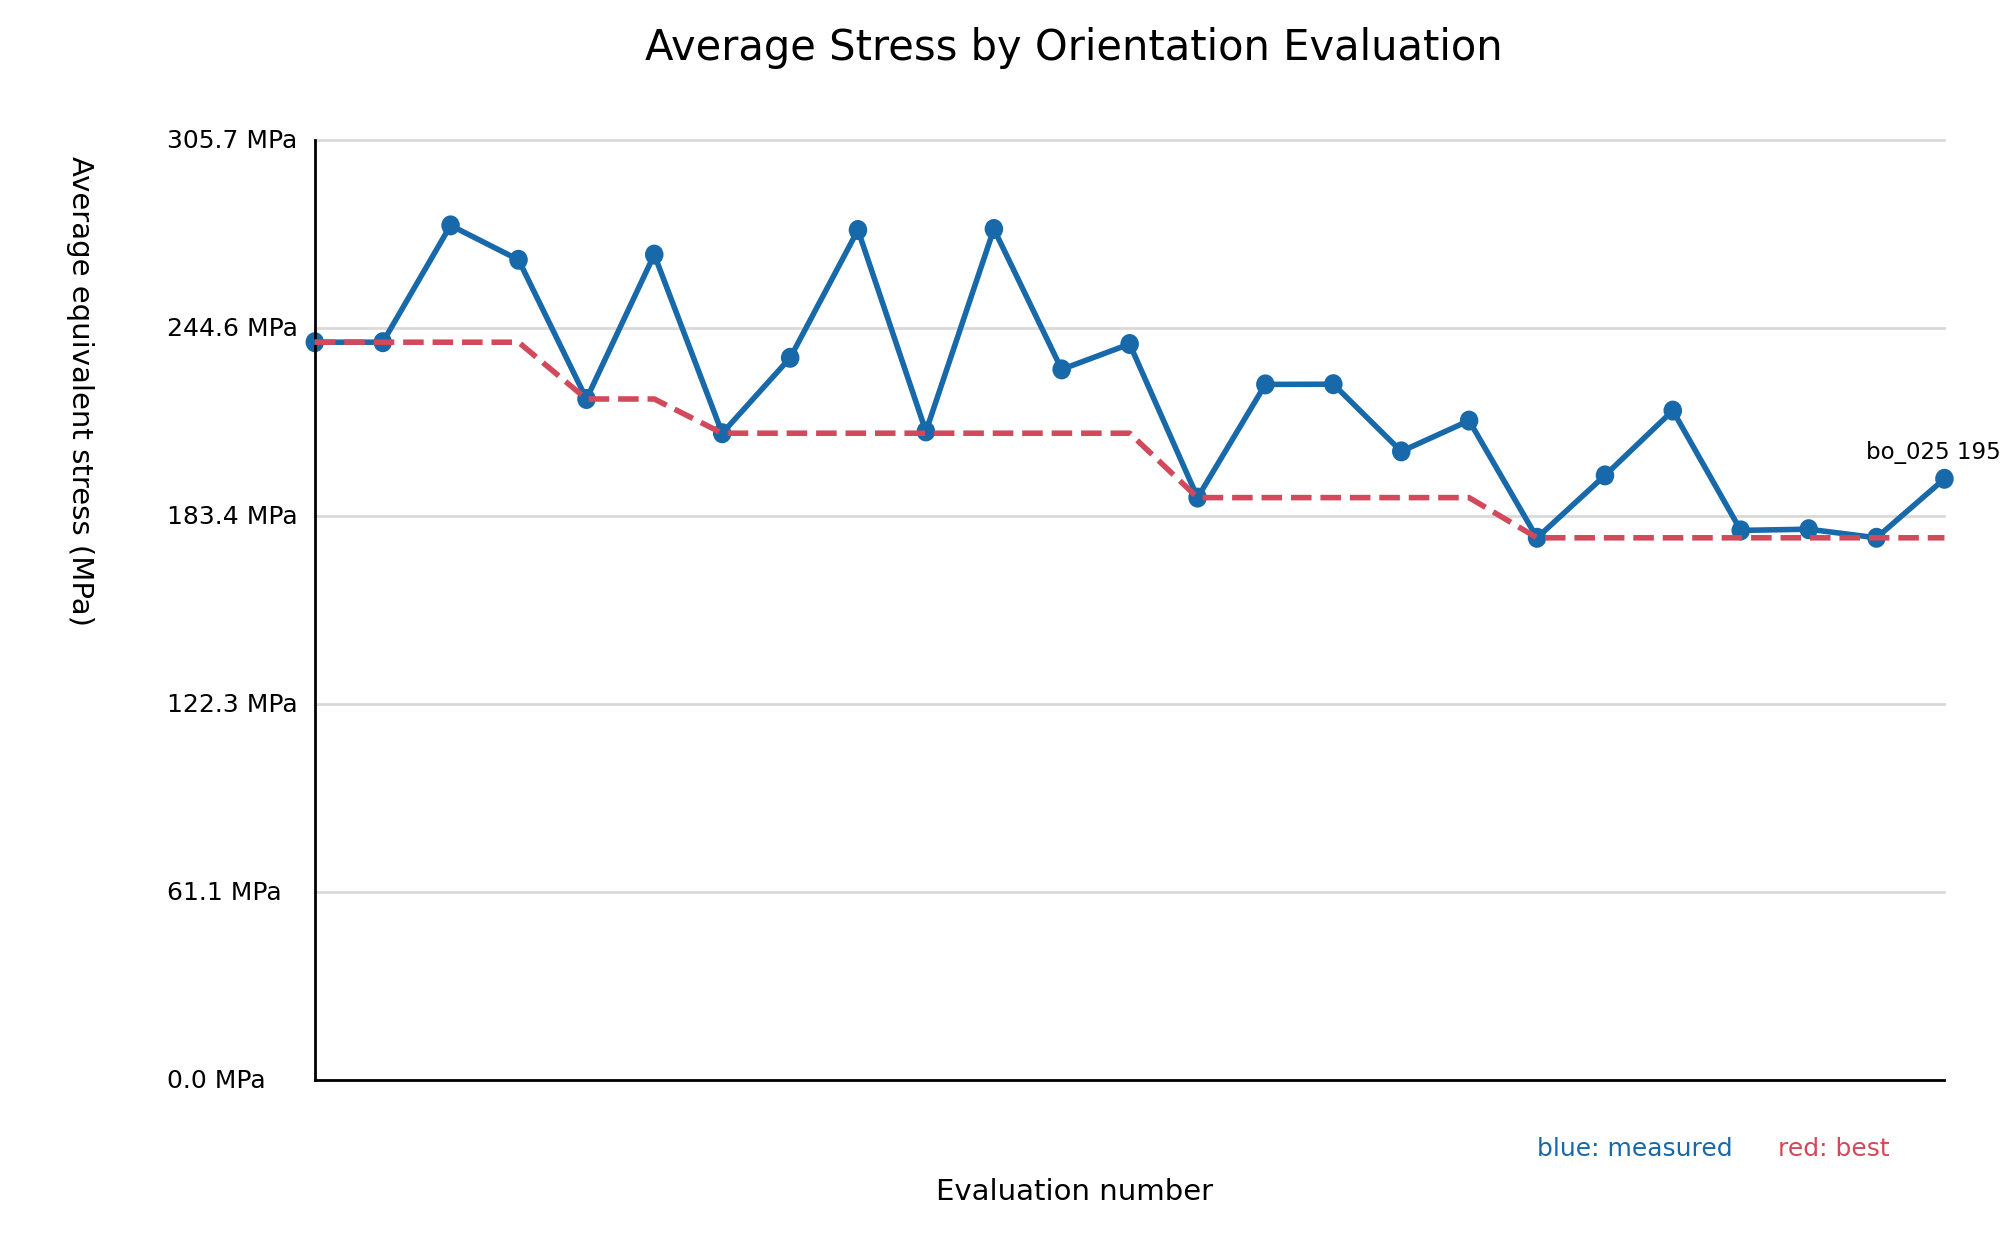
\includegraphics[width=1\columnwidth]{Figures/Results/Exhaust Manifold/results/stress_progress.png}
	\caption[The graph showing the progression of average stress over the run's iterations.]{The graph showing the progression of average stress over the run's iterations.}
	\label{fig:Exhaust Manifold Stress Graph}
\end{figure}

\begin{figure}[H]
	\centering
	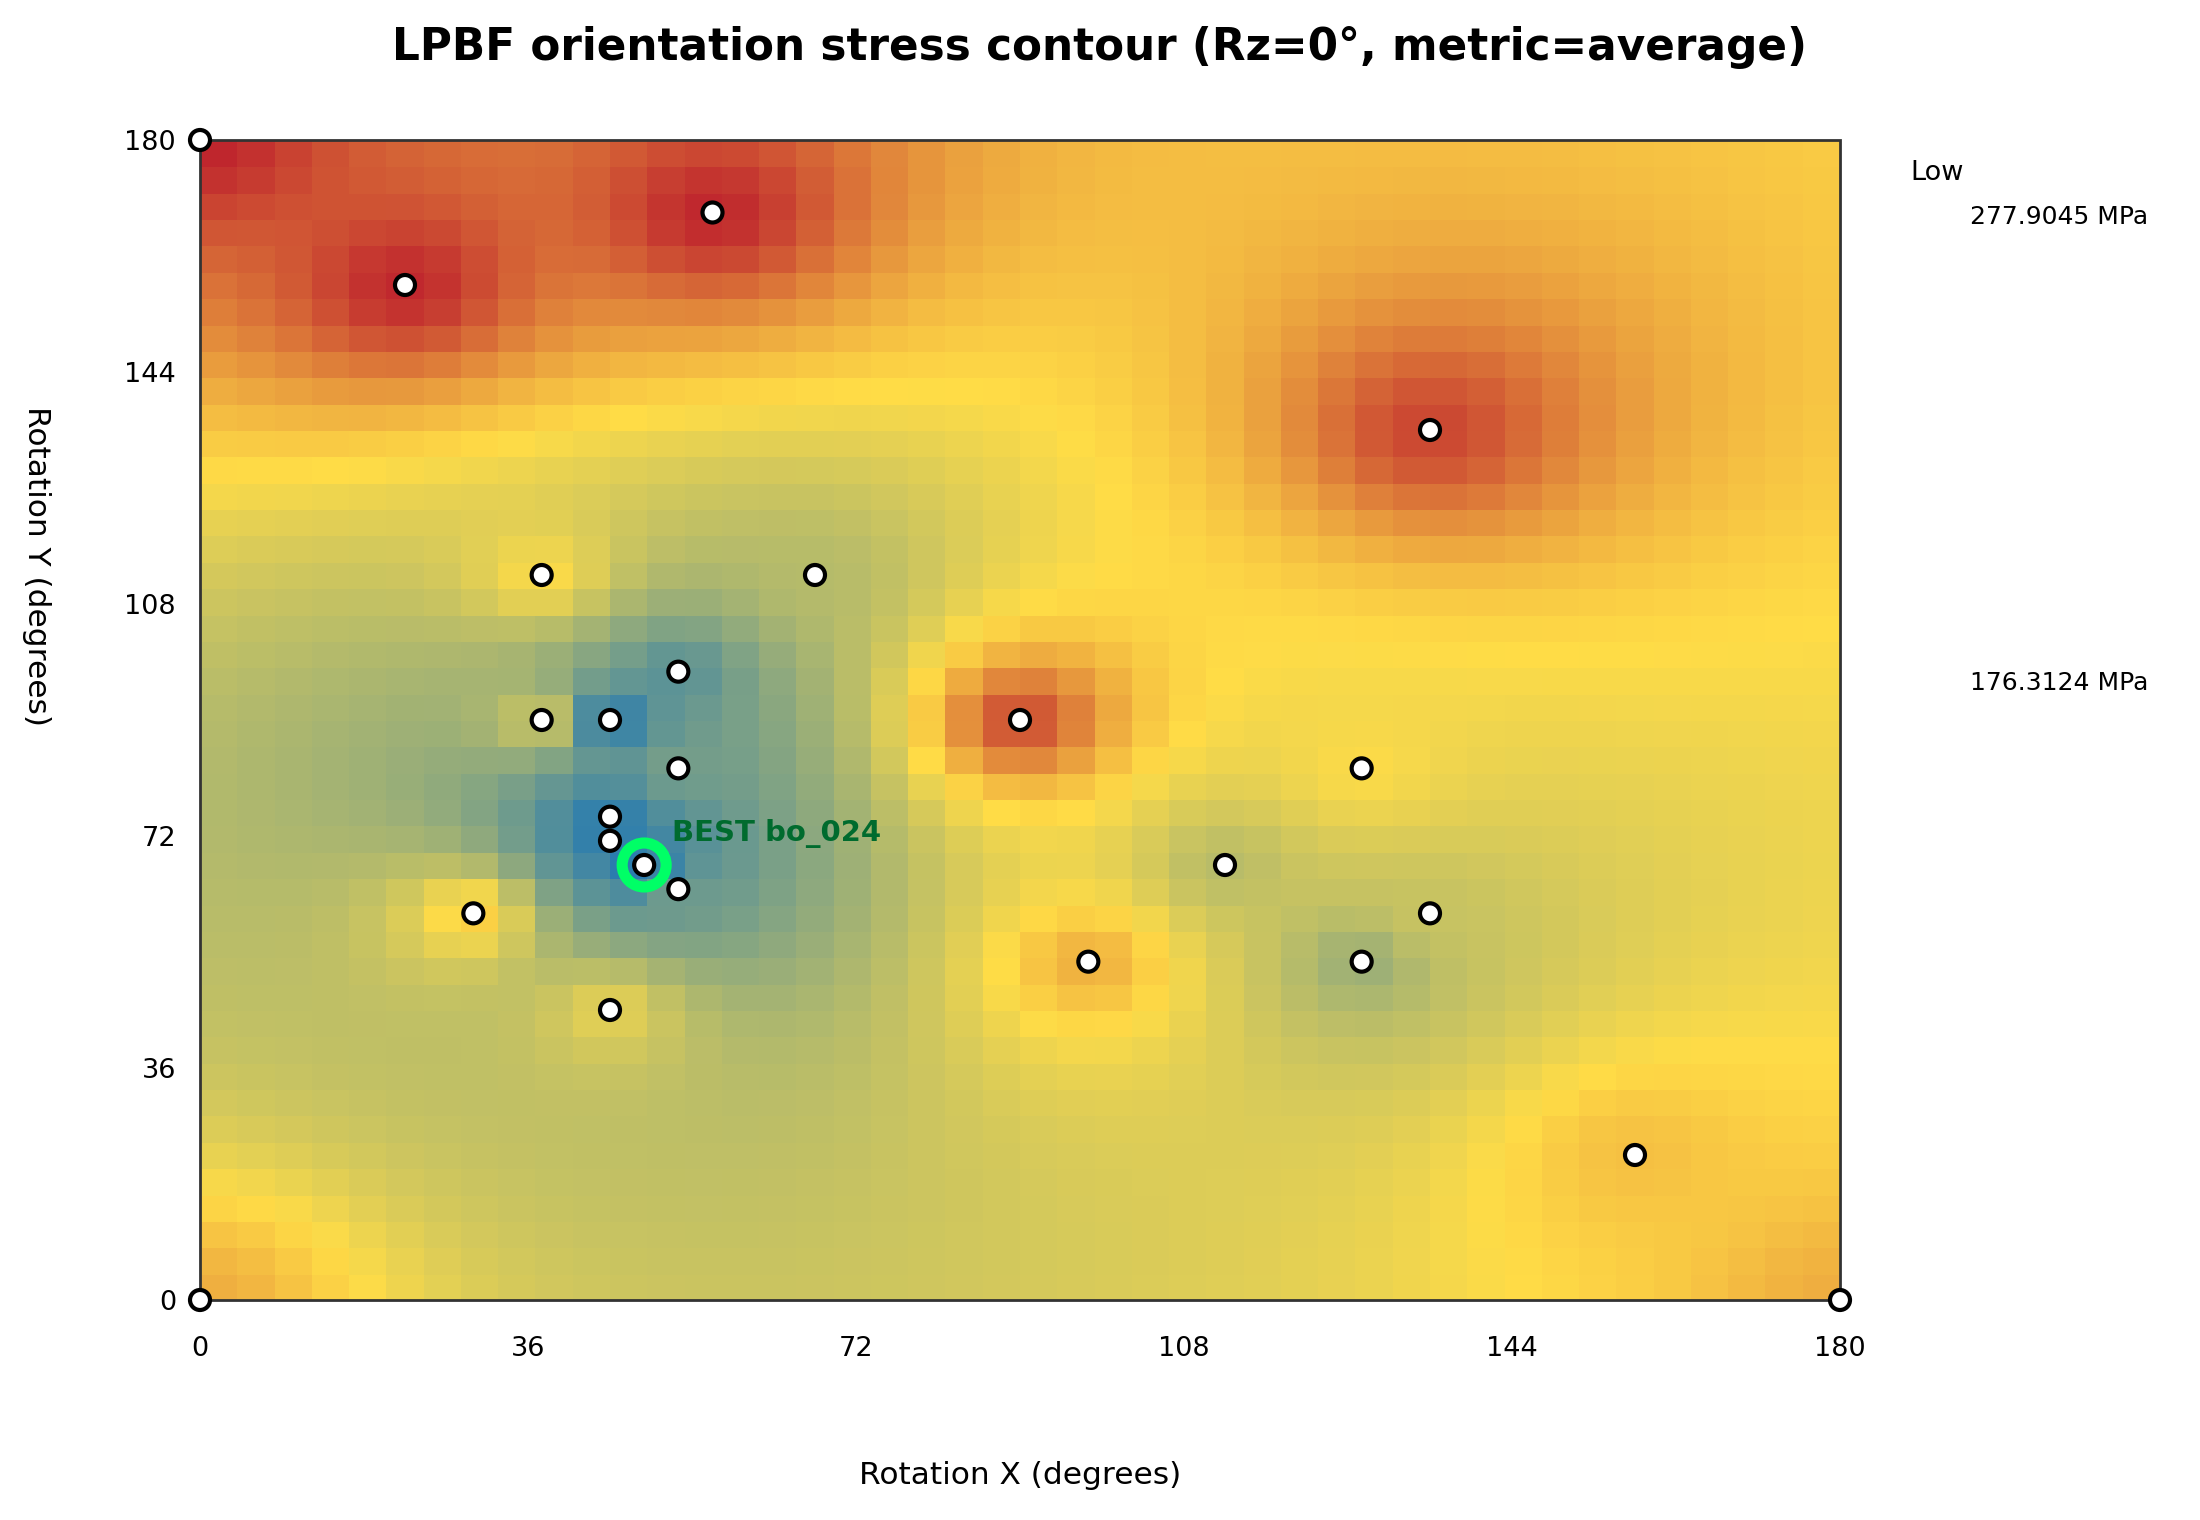
\includegraphics[width=1\columnwidth]{Figures/Results/Exhaust Manifold/results/orientation_contour_map.png}
	\caption[A contour map of the stress vs. rotation angle.  Note the data is quite sparse, so graph usefulness may be questionable.]{A contour map of the stress vs. rotation angle.  Note the data is quite sparse, so graph usefulness may be questionable.}
	\label{fig:Exhaust Manifold Stress Contour}
\end{figure}